\documentclass[letter]{article}

%% Language and font encodings
\usepackage[english]{babel}
\usepackage[utf8x]{inputenc}
\usepackage[T1]{fontenc}
\usepackage{enumitem}
\usepackage{fancyhdr}
\pagestyle{fancy}

%% Useful packages
\usepackage{amsmath, amsthm, amssymb}
\usepackage{graphicx}
\newtheoremstyle{case}{}{}{}{}{}{:}{ }{}
\theoremstyle{case}
\newtheorem{case}{}


\title{HW Template}
\author{Nicholas Silva Tee}
\lhead{Homework 3}



\begin{document}

\subsection*{Problem 1.7}
\textbf{b. } 1.6c with five states\\
\begin{figure}[h!]
	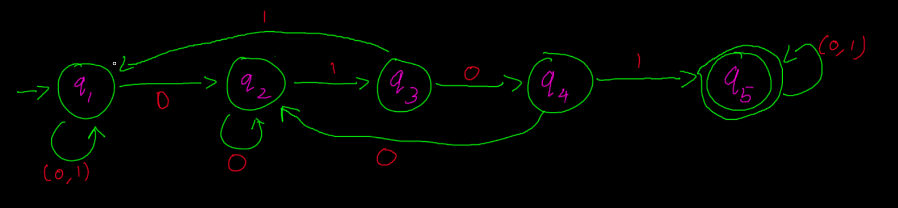
\includegraphics[scale=0.4]{7b.png}
\end{figure} \\
\textbf{c. } 1.6l with six states\\
\begin{figure}[h!]
	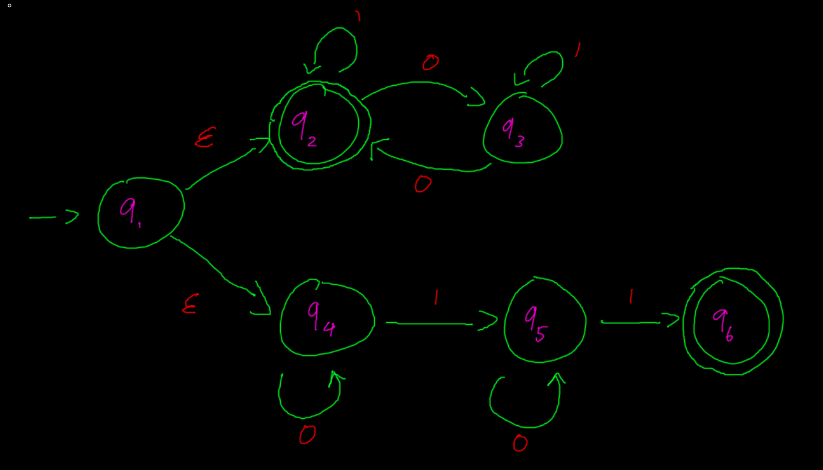
\includegraphics[scale=0.4]{7c.png}
\end{figure} \\
\textbf{d. } The language \{0\} with two states \\
\begin{figure}[h!]
	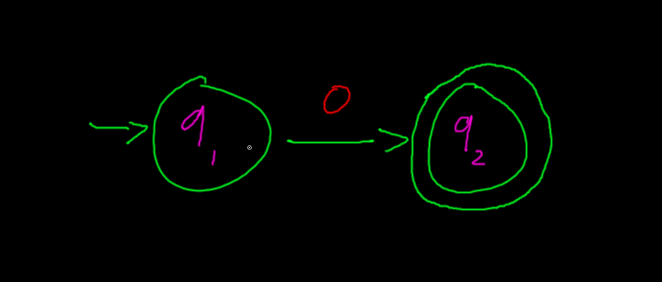
\includegraphics[scale=0.4]{7d.png}
\end{figure} 
\newpage
\textbf{e. } The language $0^*1^*0^+$ with three states\\
\begin{figure}[h!]
	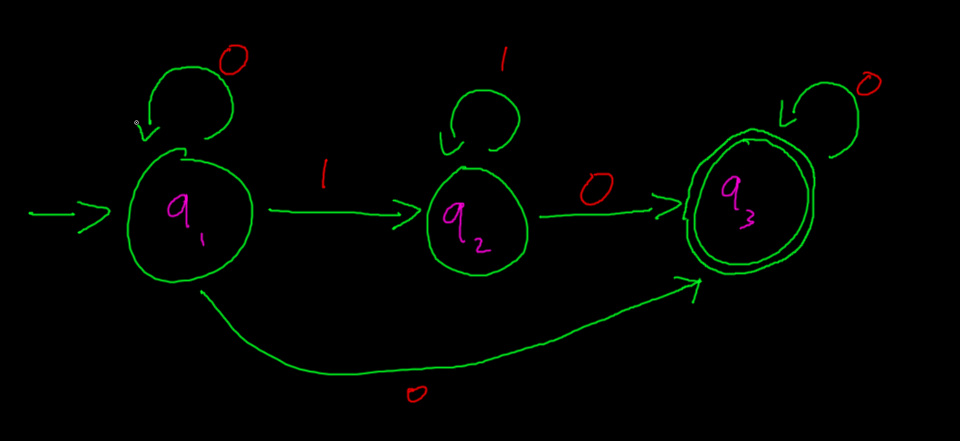
\includegraphics[scale=0.4]{7e.png}
\end{figure} \\
\textbf{g. } The language $\{\epsilon\}$ with one state\\
\begin{figure}[h!]
	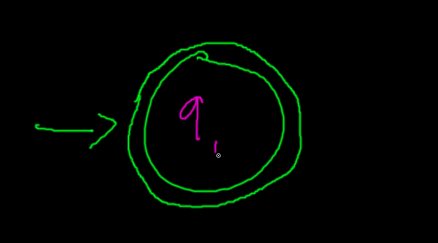
\includegraphics[scale=0.4]{7g.png}
\end{figure} \\
\textbf{h. } The language $0^*$ with one state\\
\begin{figure}[h!]
	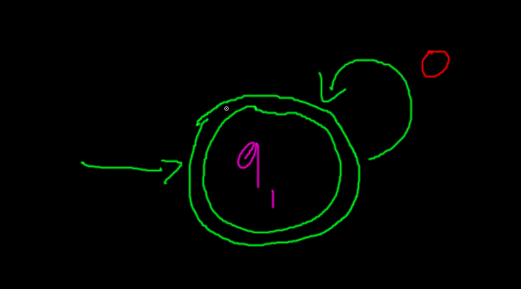
\includegraphics[scale=0.4]{7h.png}
\end{figure} \\
\newpage
\subsection*{Problem 1.13}
\begin{figure}[h!]
	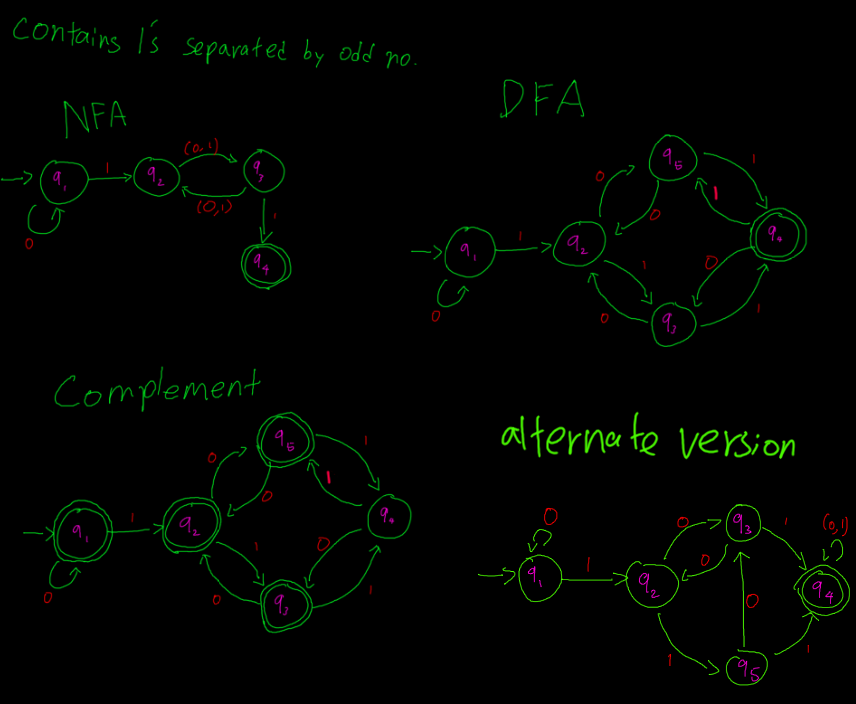
\includegraphics[scale=0.4]{13.png}
\end{figure} 
The complement that I created would not work with "1101". So I created an alternate version. However, that version does not work with the string "1001001". I not think that it is possible to create a working DFA with only 5 states.
\subsection*{Problem 1.32}
We can create a DFA called $M_B$ that will look at the "carry" of the additions. There will be 2 states $q_0$ and $q_1$ for the binary carry. This can be denoted as $q_i$ such that $i = \{0,1\}$ \\
$M_B$ definition: \\
$Q: \{q_0,q_1,q_2\}$ \\
$\Sigma: \Sigma_3$ \\
$\delta$ can be shown as: \\
\[
	\delta(q_i,[a,b,c]) = 
    \begin{cases}
    q_{(a+b+i)/2} &\text{if } i \in \{0,1\} \text{ and } c = (a+b+i) \mod 2 \\
    q_2 &\text{if } n \text{ else}
    \end{cases}
\]
$q_0$ is the start state \\
$F: \{q_2\}$
\newpage
\subsection*{Problem 1.36}
DFA's can easily be constructed for the different cases of n. two example are if n = 3 and n = 5 \\
\begin{figure}[h!]
	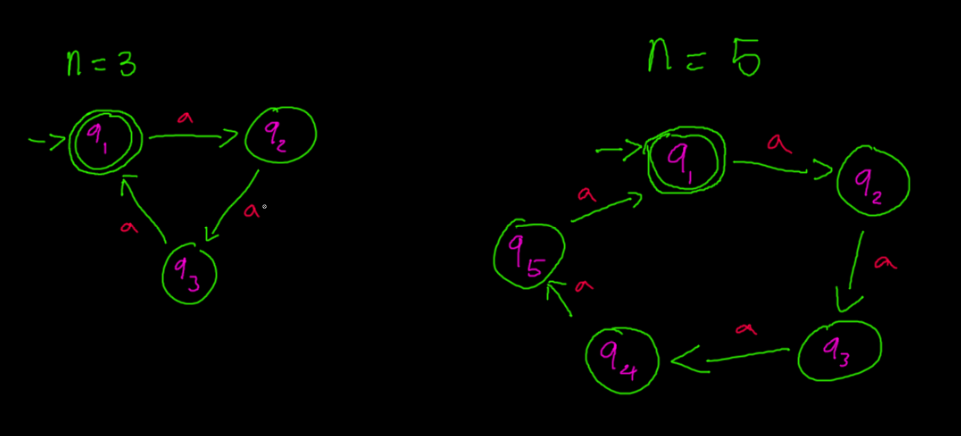
\includegraphics[scale=0.4]{36.png}
\end{figure} \\ 
This pattern can be created for any such $n \geq 1$. Which means that the language $B_n$ can be considered as regular.
\subsection*{Problem 1.37}
To show that $C_n$ is a regular language, we can show that it is possible to create a DFA for $C_2$. \\
\begin{figure}[h!]
	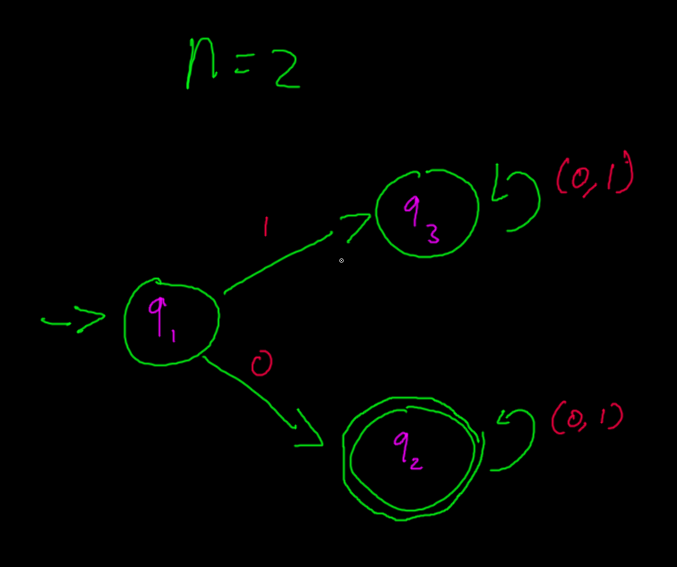
\includegraphics[scale=0.4]{37.png}
\end{figure} \\
\newpage
\subsection*{Problem 1.41}
We can assume that the states that hold the language A and B are regular. We can denote these two languages as $M_A$ and $M_B$
We can define the DFA of the perfectShuffle language as $M$. The formal defenition of $M$ can be shown as: \\
$Q: Q_A \cdot Q_B \cdot \{A,B\}$ \\
$\Sigma: \Sigma_A \cup \Sigma_B$ \\
$F: F_A \cdot F_B \cdot \{A\}$ \\
$\delta((x,y,A),a) = (\delta_A(x,a),y,B)$ \\
This shows that if the language $M_A$ is at $x$, then the language $M_B$ is at $y$ and $M_A$ contains the character that has been read next. Once the next character has been read, we can then change the language $M_A$ to $\delta_A(x,a)$ showing that the next character to be read will be in $M_B$
\end{document}










